\section{Problem\'{a}tica a Resolver}
	\subsection{Planteamiento del Problema}
	 
		La gran cantidad de veh\'{i}culos automotores que circulan en las diferentes \'{a}reas
	de San Jos\'{e}, que de acuerdo con el peri\'{o}dico La	Naci\'{o}n esta
	cantidad ronda los 260 mil veh\'{i}culos y unos 19 mil autobuses, provocan d\'{i}a a d\'{i}a embotellamientos que aumentan el tiempo requerido para ir de un punto a otro, as\'{i}
	como el consumo de combustible y por ende las emisiones de gases contaminantes.
	La situaci\'{o}n se presenta m\'{a}s alarmante cuando el mismo alcalde de San Jos\'{e}, el
	se\~{n}or Johnny Araya afirma que la cantidad de autos mencionados
	anteriormente ocupan un 70\% del espacio vial en la capital, pero \'{u}nicamente trasladan el 30\% del mill\'{o}n de personas que ingresan a San Jos\'{e} todos los d\'{i}as.\cite{Villegas2012}

		De acuerdo con la entrevista realizada a Iver Brade Monge, del Centro de
	Control de Tr\'{a}nsito del MOPT,  actualmente en Costa Rica se cuenta con un
	sistema centralizado para el control de los sem\'{a}foros, no obstante el proceso
	es manual y debe ser realizado por los operadores del mismo, los cuales de
	acuerdo con las estimaciones que realicen se aumenta o disminuye el tiempo de duraci\'{o}n de la luz verde del sem\'{a}foro, utilizando datos brindados por los contadores o c\'{a}maras localizados dentro de la red de sem\'{a}foros. Los datos de los contadores se emplean para determinar como aumenta o disminuye la cantidad de autom\'{o}viles que para por una determinada intersecci\'{o}n, mientras que las c\'{a}maras se emplean para poder visualizar la existencia o no de congestiones en las calles.
	
		El no disponer de una flu\'{i}da circulaci\'{o}n dentro de estas \'{a}reas
		responde a diferentes motivos, unos son culturales tal como lo menciona el autor de la
	nota anterior: \textit{''�algunos choferes agravan los atascamientos debido a
	maniobras indebidas, al ignorar la luz roja de los sem\'{a}foros o cuando irrespetan las
	zonas prohibidas para estacionarse\ldots La gente no aplica la cortes\'{i}a, no
	tiene paciencia y todo eso va perjudicando.''}  \citeA{Villegas2012}
	
		Por otro lado, tambi\'{e}n se deben a la gran cantidad de automotores
		que pasan por estas zonas, aspecto que se ve afectado de cierta forma por
		problemas de legislaciones en esta materia las cuales viven cambiando por
		decisiones gubernamentales, tal y como ocurri\'{o} en junio del
		2009 periodo durante el cual se dio la eliminaci\'{o}n, temporal, de la restricci\'{o}n vehicular para
	ingresar a San Jos\'{e} causando un aumento, para ese tiempo, del 25\% de
	veh\'{i}culos con personas que trataban de llegar a sus destinos dentro de la
	capital. Con eso no s\'{o}lo se dio incremento de automotores, sino que
	tambi\'{e}n se dieron aumentos en la duraci\'{o}n de las horas de mayor
	concentraci\'{o}n de los autom\'{o}viles y que de acuerdo con datos de
	ingenier\'{i}a de tr\'{a}nsito se estaban perdiendo entre un 10\% y 30\% en la
	disminuci\'{o}n del tiempo empleado por los autom\'{o}viles, as\'{i} como
	dejarse de obtener un ahorro de \$3 millones anuales en combustible.\cite{Mata2009}
		
		No obstante, los eventos anteriores terminan vi\'{e}ndose intensificados  por la
	falta de una regulaci\'{o}n adecuada de los sem\'{a}foros. Aun contando con el sistema
	mencionado, no es seguro que se logre reducir los problemas para circular con
	fluidez dentro de los lugares m\'{a}s visitados, ya que la cantidad de veh\'{i}culos es
	cambiante, por lo cual al momento de realizar los ajustes mencionados, \'{e}sta puede estar variando de forma que se torna ineficiente la regulaci\'{o}n de dichos tiempos.
		
		Uno de los factores que m\'{a}s incide en la problem\'{a}tica del modelo actual es
	el factor humano. Si bien la capacidad de razonamiento del ser humano es
	sorprendente, est\'{a} condicionada por factores de eficiencia que var\'{i}an
	de una persona a otra, podemos notar una similitud en la capacidad de reacci\'{o}n o el
	tiempo de respuesta que puedan demostrar, ya que estos pueden no ser constantes, y naturalmente con el trabajo continuo a corto y, especialmente, a largo plazo termina dejando marcas de una eficiencia disminuida completamente a niveles que terminan siendo perjudiciales para el tema en cuesti\'{o}n debido a que los ajustes necesarios al sistema de sem\'{a}foro no se podr\'{a}n realizar de forma oportuna.
		
		Por otro lado, un sistema de sem\'{a}foros basado en redes neuronales busca
	resolver esta brecha en la eficiencia tanto de razonamiento como de tiempo de
	respuesta, ya que no resulta lo mismo que una o m\'{a}s personas vean los datos
	brindados por los sem\'{a}foros segundos despu\'{e}s y con estos tomen
	decisiones, a que los mismos sem\'{a}foros se comuniquen entre s\'{i} para conocer el estado actual de su entorno y con esto obtener una acci\'{o}n a ejecutar.
		
		Es com\'{u}n que sucedan situaciones en las que, por ejemplo, unos carros que se
	ponen en marcha luego de haber estado detenidos esperando a que cambiara la
	luz, se topen con la sorpresa de que el sem\'{a}foro de la siguiente intersecci\'{o}n
	no ha cambiado o peor a\'{u}n acaba de pasar a la luz roja, segundos antes de
	que los veh\'{i}culos alcanzaran esta intersecci\'{o}n. En ambos casos se
	est\'{a} causando que los veh\'{i}culos se detengan o pasen a marchas menores
	generando un mayor consumo de combustible ya que los motores se ven forzados a
	trabajar a revoluciones demasiados bajas. Seg\'{u}n estudios realizados por
	organizaciones,  en caso de darse un tr\'{a}fico fluido, el consumo del
	combustible aumenta acorde con la velocidad, bajo estas afirmaciones se dice
	que una reducci\'{o}n de velocidad a niveles altos, terminan causando una
	disminuci\'{o}n del consumo de combustible por ejemplo al conducir a 90km/h, en lugar de 110km/h, se logra ahorrar un 23\% del consumo de combustible. No obstante a velocidades por debajo de 20km/h, el consumo aumenta considerablemente. \cite{ConferenciaEuropeadeMinistrosdeTransporte206}
		
		
		Ahora bien, si se considera la situaci\'{o}n anterior a lo largo de una avenida,
	como la avenida segunda en San Jos\'{e}, este proceso podr\'{i}a repetirse varias
	veces. El escenario se torna peor al incluir las calles que atraviesan esta
	avenida ya que se pueden presentar escenarios similares.
		
		De esta forma, se puede notar c\'{o}mo se torna m\'{a}s compleja la regulaci\'{o}n de los
	tiempos para los sem\'{a}foros y que en cuesti\'{o}n de segundos un cambio puede
	resultar inadecuado o ineficiente debido a que por haber realizado ajustes
	para beneficiar a unos, quiz\'{a}s se perjudica a muchos m\'{a}s o en el peor de los
	casos, ninguno sale beneficiado porque existen problemas similares en lugares
	cercanos.
		
	\subsection{Problema a evaluar}	
	
	 		Existen diferentes escenarios por los cuales se puedan dar los problemas
	planteados anteriormente, para esta tesis se utilizar\'{a} como caso de estudio el
	escenario representado en la figura \ref{fig:traficoSJ} %(localizada en la
	%p\'{a}gina \pageref{fig:traficoSJ})

	\begin{figure}[htp]
		\begin{center}
			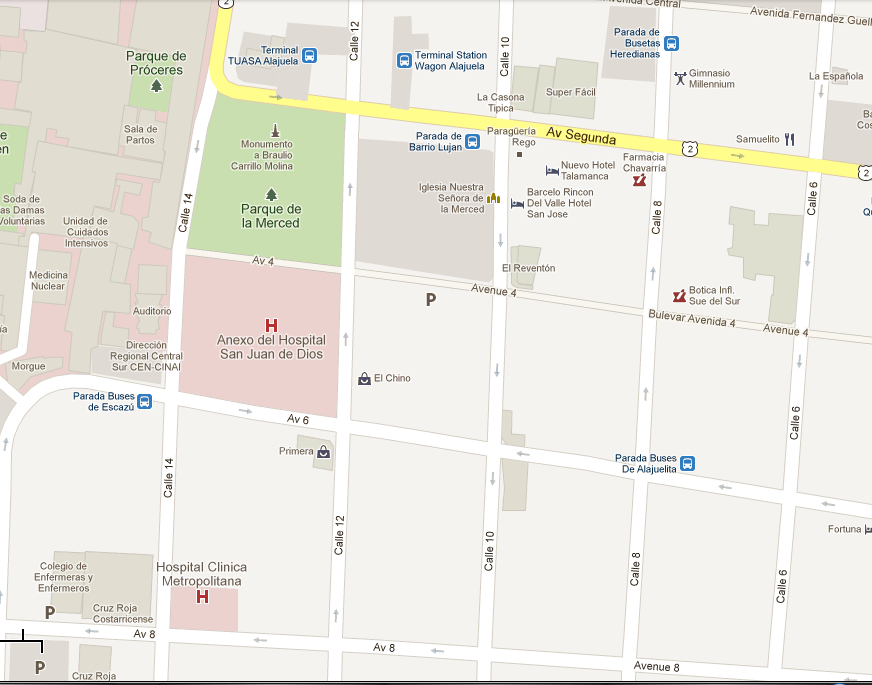
\includegraphics[totalheight=0.51\textheight]{images/trafico1}
			\caption{Diagrama de calles, San Jos\'{e} Costa Rica (Google Maps)}
			\label{fig:traficoSJ}
		\end{center}
	\end{figure}
		
		

		Basado en dicha imagen, se plantea el problema de cambio de las luces de los
	sem\'{a}foros tomando como referencia la \textbf{avenida:} 2, 4 y 8,  y las
	\textbf{calles:}
	12, 10, 8 y 6. Para este caso la avenida segunda se ve afectada fuertemente por los veh\'{i}culos automotores que quedan en medio de las intersecciones, si bien este es un problema m\'{a}s cultural, se ver\'{i}a mitigado al contar con una red de sem\'{a}foros inteligentes que tomen decisiones basados en su entorno.
	
		As\'{i} por ejemplo, al presentarse una disminuci\'{o}n del flujo de veh\'{i}culos
	automotores desde la intersecci\'{o}n de la avenida 6 y calle 10 hasta la avenida
	segunda, debido a que los sem\'{a}foros de estas est\'{a}n pasando a la luz roja,
	posiblemente se generar\'{a} una obstrucci\'{o}n en los carros que circulan a  trav\'{e}s
	de la avenida segunda. Al presentarse este escenario, muchos de los veh\'{i}culos no podr\'{a}n pasar aun cuando tengan la luz verde permiti\'{e}ndoselos.
	
		Dependiendo de las condiciones en ese momento, ya sea un alto n\'{u}mero de
	veh\'{i}culos automotores en la cercan\'{i}a o la presencia de una fuerte lluvia que
	dificulte la conducci\'{o}n, es probable que se genere un efecto en cadena el cual
	culminar\'{a} afectando, con igual o mayor rapidez, otras \'{a}reas.
	
		Otro posible escenario, es la ausencia de un n\'{u}mero significativo de
		veh\'{i}culos que est\'{a}n pasando por alguna de las calles de la intersecci\'{o}n, mientras que la
	avenida se encuentra llena o a punto de saturarse por la imposibilidad de poder
	pasar debido a la luz roja, porque otro de los sem\'{a}foros est\'{a} permitiendo paso
	a  unos cuantos veh\'{i}culos que vienen por la calle. En este caso el causar que se detengan muchos automotores por permitir pasar a unos cuantos generar\'{a} un aumento en el consumo de combustible porque estos deben arrancar o pasar a bajas velocidades.
	
		En ambos casos, es notable como una mala coordinaci\'{o}n entre los sem\'{a}foros de
	una red terminan causando estragos en las calles del pa\'{i}s. Aun contando con
	sistemas de control centralizados para el manejo de estos, no se puede
	garantizar una mejora notable en el rendimiento ya que los c\'{a}lculos son
	realizados por personas y el tiempo o consideraciones que tomen estos, pueden no ser suficientes para tomar la mejor decisi\'{o}n.
	
	
